\graphicspath{{images/}}

\section{\thesection~Introduction}
\label{sec:introduction}

% Expand motivation, describe QFA, discuss alternative approaches.

% Dummy \citet{Lawless2010} citations \citep{Heydari2016} \citep{Addinall2008}.

% The bacteria \textit{Eschericia Coli} and yeast \textit{Saccharomyces
%   cerevisae} are unicellular organisms studied as a model prokaryote
% and eukaryote respectively. They grow in colonies, where cells may (be
% clones originating from a single cell or) belong to different genetic
% strains originating from different individual cells. In favourable
% conditions, growth is exponential and this makes growth rate a major
% component of fitness; faster growing strains quickly come to dominate
% the population. Growth rate is measurable and is often used to
% determine the fitness of microbial organisms. For unicellular
% organisms, growth rate is equal to cell cycle progression
% rate. Evolutionary pressure has led to rapidly dividing organisms with
% a compact genome of essential genes. These genes have been conserved
% in other species over billions of years of evolution. The eukaryote
% \textit{S. cerevisae}, is particularly useful for the study of other
% eukaryotes such as humans.


The bacteria \textit{Eschericia Coli} and yeast \textit{Saccharomyces
  cerevisae} are unicellular organisms studied as a model prokaryote
and eukaryote respectively. They grow in colonies, where cells may (be
clones originating from a single cell or) belong to different genetic
strains originating from different individual cells. In favourable
conditions, growth is exponential and this makes growth rate a major
component of fitness; faster growing strains quickly come to dominate
the population. At a certain point growth becomes limited and a
stationary phase is reached. For unicellular organisms, growth rate is
equal to cell cycle progression rate. Evolutionary pressure has led to
rapidly dividing organisms (such as \textit{E. Coli} and \textit{S.
  cerevisae}) with compact genomes of essential genes. These genes
have been conserved in other species over billions of years of
evolution. The eukaryote \textit{S. cerevisae}, is particularly useful
for the study of other eukaryotes such as humans.

The growth rate of microbial organisms is measurable and is often used
to determine fitness. In experiments, cell cultures are commonly grown
in two types of medium. In spot tests (phenotypic array), cultures are
pinned or inoculated on the surface of a solid agar containing
nutrients. In liquid culture assays, cultures are mixed in a liquid
medium containing nutrients. In both cases cultures are incubated and
growth is observed. Identical strains can grow differently between the
two mediums and disagreement in fitness estimates is currently an
issue \citet{Baryshnikova2010} (I couldn't find a paper specifically
talking about this issue but they have a correlation plot Fig2a where
correlations are worse with a liquid culture study by Jasnos and
Korona; in fact the Baryshnikova paper Fig3c seems to say that they
had strong correlation in their ``high-resolution liquid growth
profiling study''). I do not focus on this issue and exclusively study
fitness screens using solid agar.

% Where do cells grow surfaces films.

%%% Genetic interaction, SGA and QFA %%%

% Synthetic Genetic Array (SGA) and Quantitative Fitness Analysis (QFA)
% are high-throughput methods for obtaining quantitative fitness
% estimates of microbial cultures grown on solid agar
% \citep{Baryshnikova2010sga,Banks2012}.

% Fitness estimates can be used to infer genetic interaction or drug
% response and high-throughput methods allow this to be done on a
% genome-wide scale (see e.g. \citet{Costanzo2010}). In a typical
% genetic interaction study, a strain is made with a mutation in a query
% gene. Double mutants are created by introducing a second deletion in
% this strain. Typically one query gene is used per plate with
% replicates of many different deletions. By comparing the growth of
% double mutants with a control containing a neutral deletion, genetic
% interactions can be inferred. If a strain is fitter than the control
% then the deletion is said to suppress the defect of the query gene. If
% a strain is fitter than the control then the deletion is said to
% enhance the defect of the query gene. Either scenario suggests that
% the two genes interact and have a related function. Typically one
% query gene is used per plate and many replicates of each deletion are
% contained on each plate. Many plates can be analysed in
% high-throughput to explore whole genomes.


Fitness estimates can be used to infer genetic interaction or drug
response and high-throughput methods allow this to be conducted on a
genome-wide scale (see e.g. \citet{Costanzo2010,Andrew2013}). In a
typical genetic interaction screen, a strain is made with a mutation
in a query gene. Double mutants are created by introducing a second
deletion in this strain. By comparing the growth of double mutants
with a control containing a neutral deletion, genetic interactions can
be inferred. If a strain is fitter than the control then the deletion
is said to suppress the defect of the query gene. If a strain is less
fit than the control then the deletion is said to enhance the defect
of the query gene. Either scenario suggests that the two genes
interact and have a related function. Due to redundancy, single
deletions are often non-lethal. (Remove: Knock downs and conditional
mutations can also be used.) This allowed \citet{Costanzo2010} to
explore \(\sim\)75\% of the \textit{S. cerevisae} genome.


Synthetic Genetic Array (SGA) and Quantitative Fitness Analysis (QFA)
are high-throughput methods for obtaining quantitative fitness
estimates of microbial cultures grown on solid agar
\citep{Baryshnikova2010sga,Banks2012}. Typically one query gene and
replicates of deletion are contained in a rectangular array on a solid
agar plate. Many plates with different query genes and deletions can
be grown in high-throughput to explore whole genomes. I study data
from QFA which refers to quantitative estimation of fitness by
measurement and fitting of growth curves.

In a typical QFA procedure liquid cultures are incolulated onto solid
agar (containing nutrients (already mentioned above)) often with 384
cultures in 16x24 rectangular array. Initial inoculum density can be
varied to capture more or less of the growth curve. It is estimated
that dilute cultures are inoculated with \(\sim\)100 starting cells
\citep{Addinall2011}. Plates are grown in incubation. Photographs of
whole plates are taken at timepoints throughouth growth which
typically covers several days. Images are processed by Colonyzer
\citep{Lawless2010} to produce cell density estimates from the
intensity of cultures in photographs. Current analysis independently
fits the logistic growth model to the timecourse of each culture and
fitness estimates are derived in terms of the growth constant, \(r\),
and carrying capacity, \(K\).

% logistic equation.

The logistic growth model,
\begin{equation}
  \label{eq:logistic_rate}
  \dot{C} = rC\left(1 - \frac{C}{K}\right)
\end{equation}
\citep{Verhulst1845}, for a population of density \(C\), with parameters, \(r\), growth
rate and \(K\), carrying capacity, describes self-limiting growth and is currently used to
fit QFA data with an assumption of independence between cultures
\citep{Addinall2011,qfa2016}. It has the following analytical solution:
\begin{equation}
  \label{eq:logistic_solution}
  C(t) = \frac{KC_{0}e^{rt}}{K + C_{0}(e^{rt}-1)},
\end{equation}
where P is the initial population density. Measures of fitness are
commonly defined in terms of the parameters \(r\), \(K\), and initial
cell density \(C_{0}\) \citep{Addinall2011}. We hope to improve the
reproducibility of fitness estimates using a model accounting for
competition and signalling



In contrast, SGA typically uses an array of 1536 pinned cultures and
an endpoint assay of culture area to quantify growth.


QFA
collects more information about growth by taking images of plates at
points throughout the growth curve. QFA can be performed using either
the pinned cultures (used in SGA) or dilute liquid cultures
(``spots'') of lower initial cell density. Although pinned QFA allows
for more cultures per plate (1536 vs 384 in spotted), spotted QFA
allows for more accurate fitting of growth models as growth curves are
more complete (see Figure~\ref{fig:qfa_and_sga_growth_curves})
\citep{Lawless2010}. Comparison of spotted and pinned QFA cultures in
Figure~\ref{fig:qfa_and_sga_growth_curves}c shows how spotted cultures
are composed of many individual colonies which increase in size and
thickness, whereas pinned cultures are composed of a single uniform
colony which grows radially. The number of individual colonies in a
spotted culture is high enough that lag and other stochastic effects
should average out.

% Example use of QFA by Addinall telomeres.




\subsection{\thesubsection~Subsection}

\begin{Figure}
  \centering
  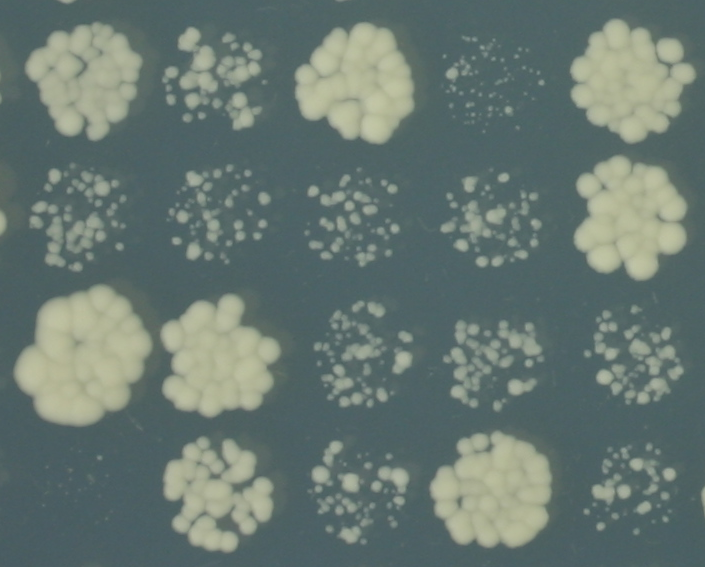
\includegraphics[width=\linewidth]{p15_section/p15_section}
  \captionof{figure}{\textbf{4x5 section of a QFA plate.} Taken from a
    16x24 format solid agar plate inoculated with dilute
    \textit{S. cerevisae} cultures.
  Image captured at \(\sim\)2.5d after inoculation and incubation at
  27\(^{\circ}C\).}
  \label{fig:p15_section}
\end{Figure}


\begin{Figure}
  \centering
  \includegraphics[width=\linewidth]{stripes/final/striped}
  \includegraphics[width=\linewidth]{stripes/final/filled}
  \captionof{figure}{\textbf{An experiment designed to examine
      competition.}\\
    A) QFA plate inocluated with a more concentrated
    \textit{S. Cerevisae} inoculum (no cells inocluated on alternative
    columns).\\
    B) Same as in A, but with strains of similar growth rate
    inoculated in the positions missing in A.}
  \label{fig:stripes_images}
\end{Figure}



%%% Local Variables:
%%% mode: latex
%%% TeX-master: "report"
%%% End:
